\paragraph{The active case with reactions.}

\textit{This section was contributed by Juliane Dannberg and Ren{\'e} Ga{\ss}m{\"o}ller}.

In addition, there are setups where one wants the compositional fields to interact with each other. One example would be material upwelling at a mid-ocean ridge and changing the composition to that of oceanic crust when it reaches a certain depth. In this cookbook, we will describe how this kind of behavior can be achieved by using the \texttt{composition reaction} function of the material model.

We will consider the exact same setup as in the previous paragraphs, except for the initial conditions and properties of the two compositional fields. There is one material that initially fills the bottom half of the domain and is less dense than the material above. In addition, there is another material that only gets created when the first material reaches the uppermost 20\% of the domain, and that has a higher density. This should cause the first material to move upwards, get partially converted to the second material, which then sinks down again. This means we want to change the initial conditions for the compositional fields:

\lstinputlisting[language=prmfile]{initial.part.prm.out}


Moreover, instead of the \texttt{simple} material model, we will use the \texttt{composition reaction} material model, which basically behaves in the same way, but can handle two active compositional field and a reaction between those two fields. In the input file, the user defines a depth and above this \texttt{reaction depth} the first compositional fields is converted to the second field. This can be done by changing the following section (the complete input file can be found in \url{cookbooks/composition-reaction/composition-reaction.prm}).

\lstinputlisting[language=prmfile]{material.part.prm.out}

\begin{figure}
  \centering
  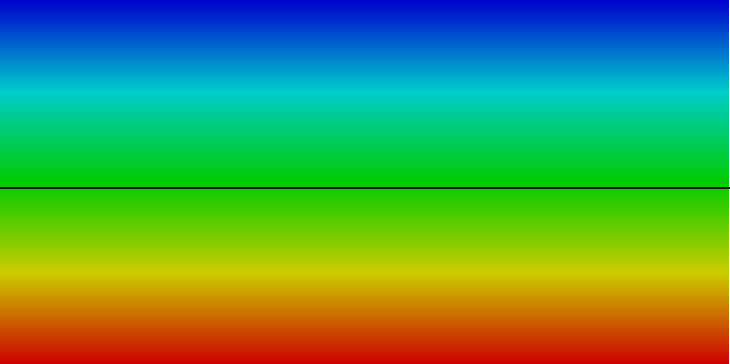
\includegraphics[width=0.3\textwidth]{0.png}
  \hfill
  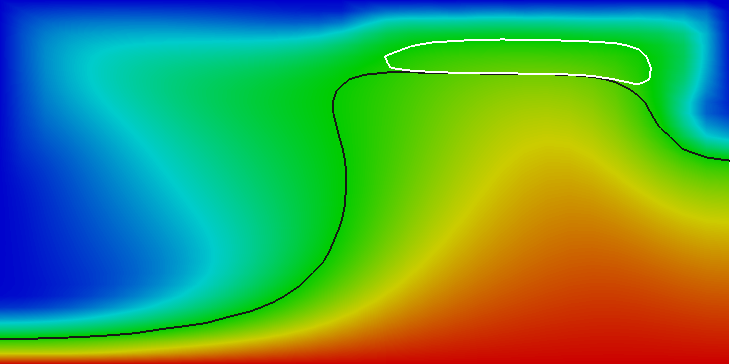
\includegraphics[width=0.3\textwidth]{2.png}
  \hfill
  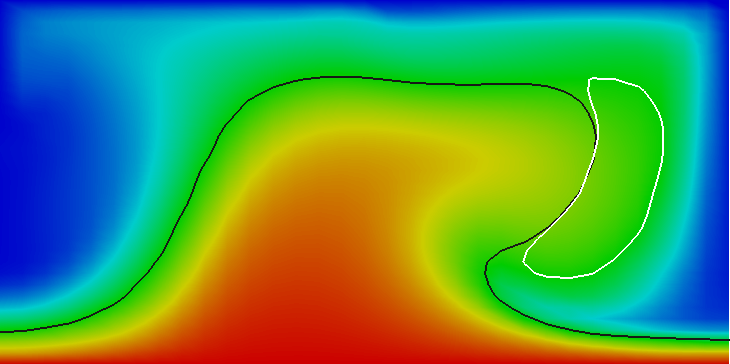
\includegraphics[width=0.3\textwidth]{4.png}
  \\[6pt]
  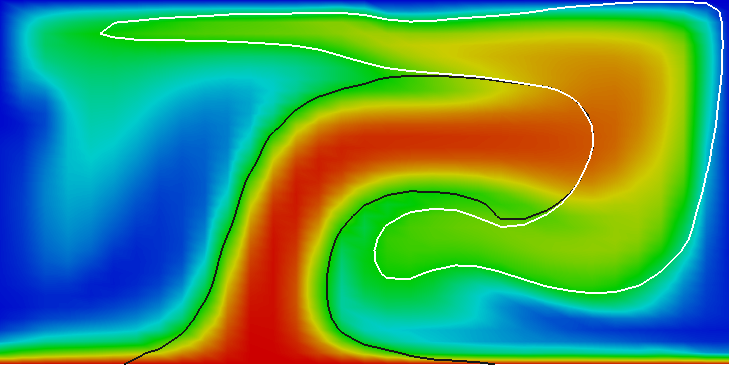
\includegraphics[width=0.3\textwidth]{8.png}
  \hfill
  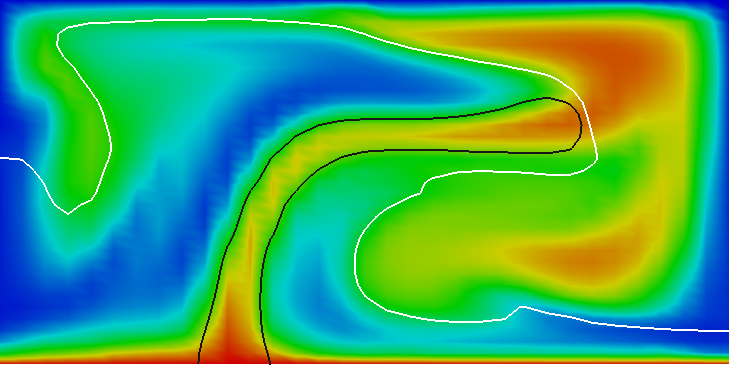
\includegraphics[width=0.3\textwidth]{12.png}
  \hfill
  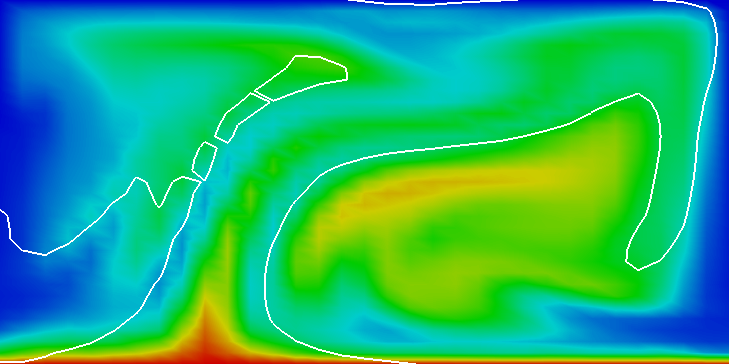
\includegraphics[width=0.3\textwidth]{20.png}
  \caption{\it Reaction between compositional fields: Temperature fields at $t=0, 2, 4, 8,
  12, 20$. The black line is the isocontour line $c_1(\mathbf x,t)=0.5$
    delineating the position of the material starting at the bottom and the white line is the    isocontour line $c_2(\mathbf x,t)=0.5$
    delineating the position of the material that is created by the reaction.}
  \label{fig:composition-reaction}
\end{figure}

Results of this model are visualized in
Fig~\ref{fig:composition-reaction}. What is visible is
that over the course of the simulation, the material that starts at the bottom
of the domain ascends, reaches the reaction depth and gets converted to the second material, which starts to sink down.
